\section{Sigma-Delta Wandler}
Der $\Sigma-\Delta$-Wandler Integriert bei jedem Taktzyklus auf oder ab, basierend auf dem $V_{out}$, so wird die Ladung von $Q_{Ci}$ immer auf $0$ gehalten. Ein digitaler-Teil zählt anschliessend die Schritte und kann so die Spannung bestimmen.
\begin{center}
	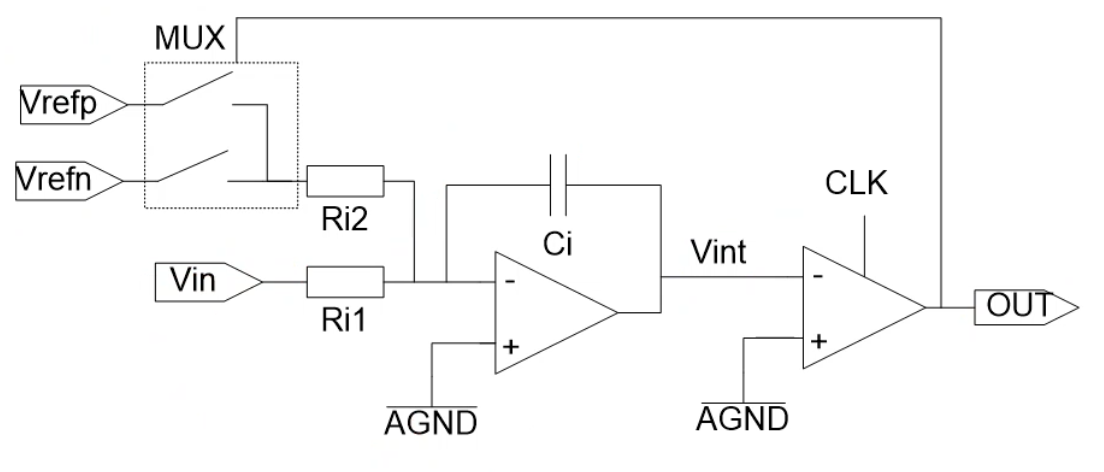
\includegraphics[width=0.8\columnwidth]{Images/sigma_delta}
\end{center}
Für $N$ Takt-Zyklen (Je höher desto grösser die Auflösung und langsamer) vom CLK und $n$ Taktperioden, in denen der Modulator-Ausgang=$1$ ist gilt:
\[
0 \approx Q_{Ci} = N\cdot \frac{C_i}{Ri_1}\cdot V_{in} +  n\cdot \frac{C_i}{Ri_2}\cdot V_{ref}-(N-n)\cdot \frac{C_i}{Ri_2}\cdot V_{ref}
\]
Wenn $Ri_1=Ri_2$ dann:
\[
0 = N\cdot V_{in}+(2n-N)\cdot V_{ref} \quad\xRightarrow[]{}\quad V_{in} = \frac{2n - N}{N}V_{ref}
\]